\chapter{Introduction}
\section{Why interpretability?}
Modern machine learning models based on deep neural networks are achieving remarkable performance in many fields. In comparison with classic machine learning technologies like decision trees, it is much harder to explain how these neural networks came to their conclusions, because they use thousands to millions of trained parameters.

Especially in the medical imaging field, it is very important that algorithms not only generate a correct diagnosis when training the algorithm, but also show that they are using the same cues in images as trained physicians. These cues are found and verified in scientific studies, and are therefore well understood and proven to be correct. A wrong diagnosis generated by a neural network reduce the confidence of physicians using the technology and can be life threatening when used without professional supervision.

\section{Image classification}
In recent years, many methods for the interpretability of deep (convolutional) neural networks have been proposed, e.g. LIME \cite{ribeiro2016should}, RISE \cite{Petsiuk2018rise}, Grad-CAM \cite{selvaraju2017grad} or DeepLIFT \cite{shrikumar2017learning}. Some example outputs of these methods are shown in F

\begin{figure}[h]
\centering
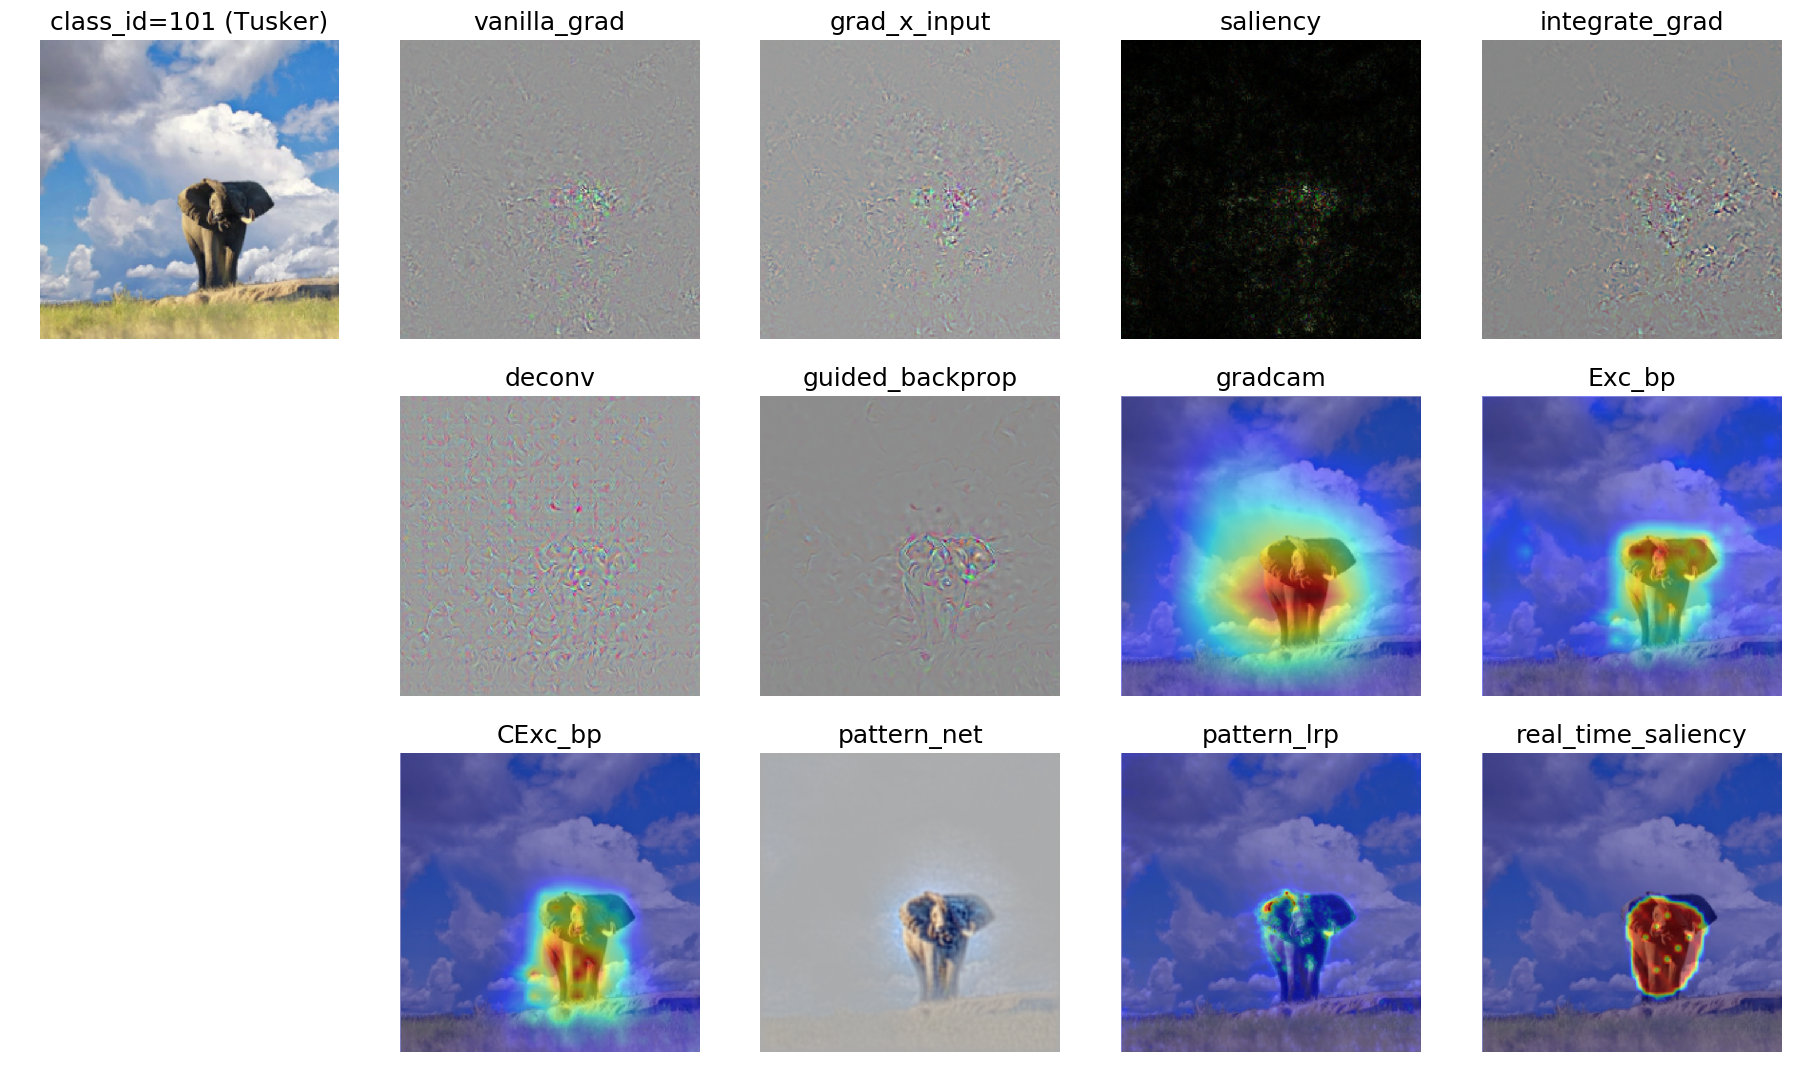
\includegraphics[width=14cm]{images/tusker_saliency.png}
\caption{Examples of some interpretability methods for image classification \cite{visualattribution}}
\label{classification_methods}
\end{figure}

These methods focus on providing explanations and interpretability of classification problems for datasets like ImageNet \cite{imagenet_cvpr09} or MNIST \cite{lecun1998gradient}. Classification means that an algorithm can tell what is displayed on an image, e.g. if and what kind of disease is visible on a x-ray or MRI scan.

\section{Image segmentation}
Image segmentation is different from classification in the way that the algoriths do not detect what is visible on a picture, but instead mark a region (the segment) in an image where it thinks something is visible. For example in self driving cars, it is important to know where another car or a pedestrian is in front of the car is. 

In the medical imaging field, one applications is the segmentation of tumors in MRI scans.

\section{Interpretability on image segmentation}
The interpretability of image segmentation task is nearly inexistent. In many cases this is understandable, because the interpretability methods would generate an image very similar to the actual segment. For example, in detecting pedestrians for self driving cars, the interpretability method would just mark the pedestrian. Only in cases where the network has not yet reached a good accuracy, other pixels in the image would be marked by the method.

In other fields like medical imaging, it is possible or even desirable that a neural network looks at other parts of an image to decide if a part should be segmented. An example for this is the search for tumors on MRI scans of the human brain. The human brain is physically symmetric. When a tumor is growing on one side of the brain, the brain is no longer symmetric. A physician and possibly also neural networks can use this property to detect and segment tumors.

\section{Goals}
The goal of this thesis is to take the existing methods for image classification and modify them so they can work on image segmentation tasks. This includes the following tasks:
\begin{itemize}
    \item Research existing methods for image classification
    \item Asses if the found methods can be modified for image segmentation
    \item Modify the methods for image segmentation
    \item Build and train a neural network on the BraTS brain tumor segmentation dataset
    \item Apply the modified methods on the trained neuronal network
    \item Analyze, evaluate and discuss the results
    \item Build a reusable Python library so other developers can easily use our modified messages
\end{itemize}

The second goal is providing the customer with images and visualization for use in their teaching material.

See appendix A for the full requirements specification.

\section{Customer}
The customer of this thesis is Mauricio Reyes and his team from the medical faculty of the University of Bern. Mr. Reyes is head Healthcare Imaging A.I. This thesis should help him and his team of master and PHD students to better understand the models they are developing.

\section{Source Code}
The source code of the thesis is available on GitHub:
\begin{itemize}
    \item Thesis source code (mostly jupyter notebooks): \url{https://github.com/andef4/thesis-code}
    \item Python library source code: \url{https://github.com/andef4/interpret-segmentation}
    \item Latex source for this document: \url{https://github.com/andef4/interpret-segmentation}
\end{itemize}

All source code is licensed under the permissive MIT license.


\chapter{Interpretability methods}
\section{Whitebox and blackbox methods}
Generally there are two types of methods for interpretability: Blackbox and whitebox. Blackbox methods like LIME or RISE do not need insight into the underlying model and can therefore be used on arbitrary network architectures and even non-deep learning technologies like decision trees.

Whitebox methods need to have access to the underling model (e.g. weights and activation values in a neural network), because they analyze a certain part of the network.

\section{Methods overview}

\begin{tabular}{| p{7cm} | p{2.5cm} | p{6cm} | }
\hline
\textbf{Method} & \textbf{Blackbox method} & \textbf{PyTorch implementation available} \\ \hline

RISE\cite{Petsiuk2018rise} & Yes & Offical implementation is PyTorch \\ \hline
LIME\cite{ribeiro2016should} & Yes & No but feasible \\ \hline
Layer-wise Relevance Propagation (LRP) & No & Yes, but missing batch normalization\cite{lrppytorch} \\ \hline
DeepLIFT\cite{shrikumar2017learning} & No & Initial implementation in SHAP\cite{NIPS2017_7062} \\ \hline
Grad-CAM (Selvaraju 2017) & No & Many implementations \\ \hline
Meaningful Perturbation (Fong 2017)\cite{fong2017interpretable} & Yes & Implementation exitst \cite{fong2017implementation} \\ \hline

Prediction Difference Analysis \cite{todo} & ? & ? \\ \hline
PatternNet & ? & ? \\ \hline
SHAP DeepExplainer\cite{NIPS2017_7062} & No & No \\ \hline
SHAP KernelExplainer\cite{NIPS2017_7062} & Yes & Yes \\ \hline

Guided Backpropagation  & No & ? \\ \hline
Excitation Backprop (Zhang 2016)\cite{todo} & No & ? \\ \hline


\end{tabular}

% many implementations: https://github.com/yulongwang12/visual-attribution
% https://github.com/marcoancona/DeepExplain/blob/master/docs/comparison.png


% Poulin'06 Additive
% Baehrens'10 Gradient
% Symonian'13 Gradient
% Landecker'13 Contrib Prop
% Zeiler'14 Deconv
% Zeiler'14 Occlusions
% Caruana'15 Fitted Additive
% Haufe'15 Pattern
% Zhou'16 GAP
% Sundarajan'17 Int Grad

\section{Method selection}
The initial selection of methods contain RISE, LIME and Grad-CAM.

LIME: Widly cited.
RISE: Proposed enhancement of LIME
Grad-CAM: Widly cited, many implementations as indicator of popularity and quality.

There are many methods, quite a few of them with PyTorch implementation.
=> visual attribution with generic code for multiple methods
If the modification of these methods for image segmentation is successful, additional methods will be selected.

\section{LIME}

LIME \cite{ribeiro2016should} (Local Interpretable Model-Agnostic Explanations) is a black box interpretability method. Like all black box methods, LIME randomly changes features in the input data to detect which feature is relevant for a specific classification.

In the case of image classification, LIME does not modify single pixels, because this would generate too many different versions of the input.
Instead, LIME generates superpixels.

\begin{figure}[H]
    \centering
    \begin{subfigure}[t]{.35\textwidth}
        \centering
        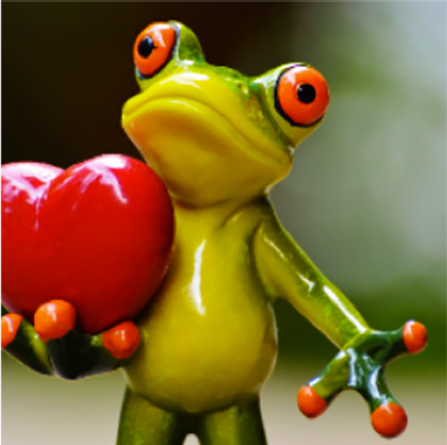
\includegraphics[width=\linewidth]{chapters/02_methods/images/frog1.png}
        \caption{Original image}
    \end{subfigure}\hspace{1.5cm}%
    \begin{subfigure}[t]{.35\textwidth}
        \centering
        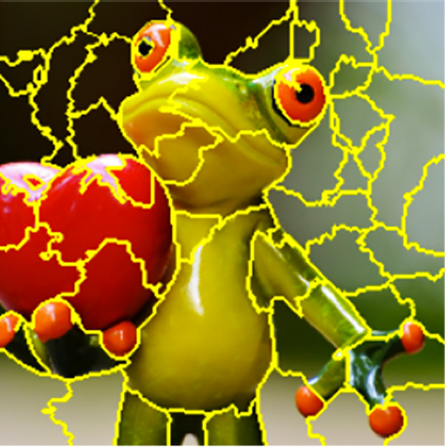
\includegraphics[width=\linewidth]{chapters/02_methods/images/frog2.png}
        \caption{Original image overlaid with superpixel boundaries}
    \end{subfigure}
    \caption{Superpixels generated for an input image. Superpixels are the features LIME analyzes to detect if they are relevant for the classification \cite{limeoreilly}.}
    \label{lime_superpixel}
\end{figure}


Superpixels are continuous regions on an image with a similar color. In the Python reference implementation, LIME uses the Quick Shift \cite{vedaldi2008quick} clustering algorithm to generate these superpixels. Figure \ref{lime_superpixel} shows superpixels overlaid on an example image.

\begin{figure}[H]
\centering
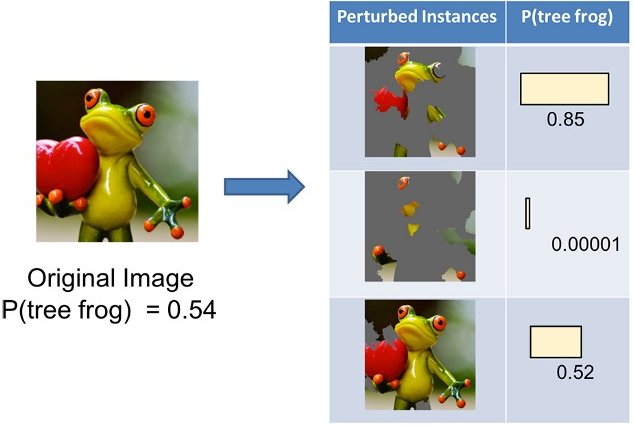
\includegraphics[width=8cm]{chapters/02_methods/images/lime1.jpg}
\caption{Left: Original image with detected class and probability. Right: Perturbed images generated by randomly turning off superpixels and their probability for the specific class.}
\label{lime_perturbed}
\end{figure}

In the next step, LIME generates input images by turning off multiple randomly selected superpixels. Turning off in this case means setting the color inside the superpixel to gray. The right image of Figure \ref{lime_perturbed} shows some examples of deactivated superpixels. The generated input images are then passed through the neural network and the changed probabilities of the relevant class(es) are recorded.

\begin{figure}[H]
\centering
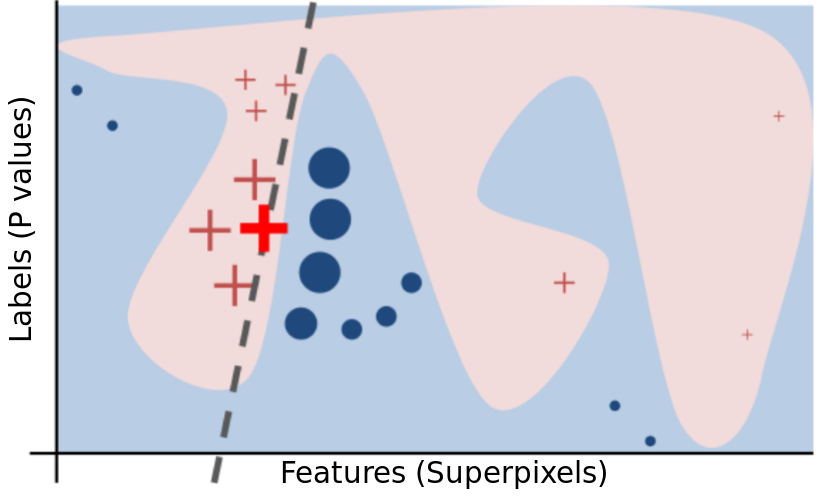
\includegraphics[width=8cm]{chapters/02_methods/images/lime2.png}
\caption{
The light red and blue background of the image represent the non-linear function of the underlying model.
The bright red cross represents the image that is explained. The smaller red crosses and blue circles represent
perturbed instances of image. The size of these symbols show the distance to the unchanged image. The x-axis represents the features, in the case of images these are the superpixels. The y-axis represents the output label of the neural network. The dashed line shows the fitted linear model.}
\label{lime_linear_regression}
\end{figure}

As a last step, LIME trains a linear regression model (Figure \ref{lime_linear_regression}) on this data: Superpixels represented as a binary vector on the x-axis and the corresponding neural network output for the specific class on the y-axis. The samples are weighted by distance to the original sample, because a linear model is trained which is accurate in the local environment of the unchanged image, but not further away because the underlying model is not linear. The coefficients of the linear model represent how important every superpixel is for the correct classification of the model.

For visualization, the coefficients are sorted by their value. Based on the superpixel count parameter given to LIME, the most important superpixels are drawn, all other superpixels are grayed out. 

Figure \ref{lime_dog} shows a visualization for three classes on a complex input image. Alternatively, the superpixel cluster is drawn over the input image with transparency.

\begin{figure}[H]
    \centering
    \begin{subfigure}[t]{.23\textwidth}
        \centering
        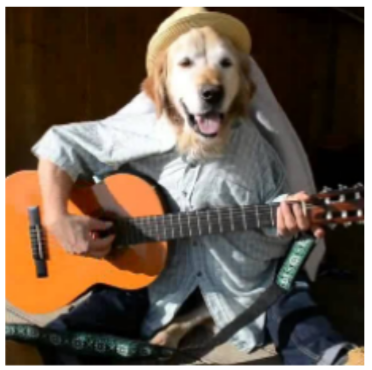
\includegraphics[width=\linewidth]{chapters/02_methods/images/lime_dog_1.png}
        \caption{Original image}
    \end{subfigure}\hfill%
    \begin{subfigure}[t]{.23\textwidth}
        \centering
        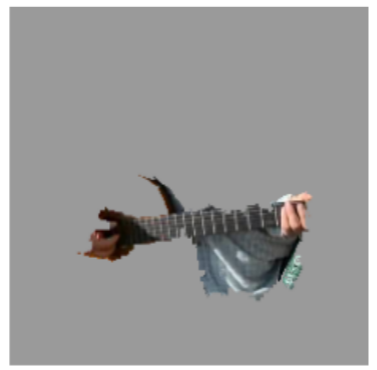
\includegraphics[width=\linewidth]{chapters/02_methods/images/lime_dog_2.png}
        \caption{Explain class "Electric guitar" (p=0.32)}
    \end{subfigure}\hfill%
    \begin{subfigure}[t]{.23\textwidth}
        \centering
        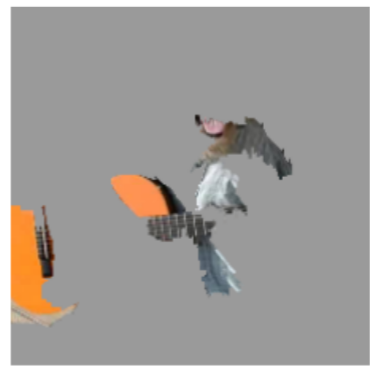
\includegraphics[width=\linewidth]{chapters/02_methods/images/lime_dog_3.png}
        \caption{Explain class "Acoustic guitar" (p=0.24)}
    \end{subfigure}\hfill%
    \begin{subfigure}[t]{.23\textwidth}
        \centering
        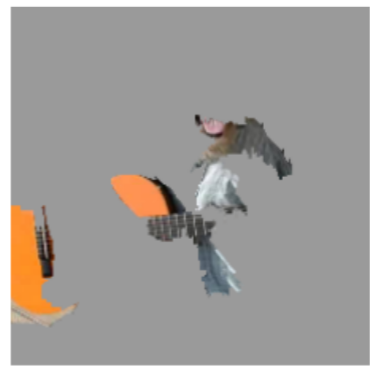
\includegraphics[width=\linewidth]{chapters/02_methods/images/lime_dog_3.png}
        \caption{Explain class "Labrador" (p=0.21)}
    \end{subfigure}
    \caption{Explaining the top 3 classes on an example image with LIME. The used neural network architecture is Inception trained on ImageNet \cite{ribeiro2016should}.}
    \label{lime_dog}
\end{figure}

\section{RISE}

Like LIME, RISE\cite{Petsiuk2018rise} is a black box method and works by manipulating of the input images.

Instead of superpixels, RISE generates masks that are applied to the input images by multiplying the mask with the input image pixel values. Figure \ref{rise_mask0} and Figure \ref{rise_mask1} show two RISE masks applied to the same input image.

\begin{figure}[H]
    \centering
    \begin{subfigure}[t]{.32\textwidth}
        \centering
        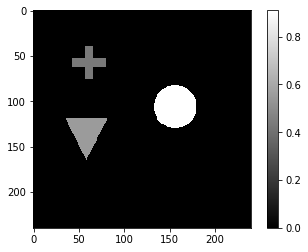
\includegraphics[width=\linewidth]{chapters/02_methods/images/rise/rise_original.png}
        \caption{Original image}
    \end{subfigure}\hfill%
    \begin{subfigure}[t]{.32\textwidth}
        \centering
        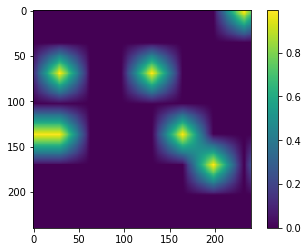
\includegraphics[width=\linewidth]{chapters/02_methods/images/rise/rise0_mask.png}
        \caption{RISE mask}
    \end{subfigure}\hfill%
    \begin{subfigure}[t]{.32\textwidth}
        \centering
        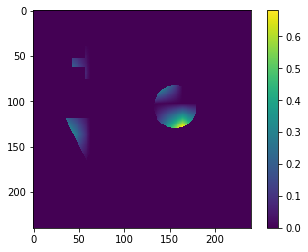
\includegraphics[width=\linewidth]{chapters/02_methods/images/rise/rise0_applied.png}
        \caption{RISE mask applied to original image by multiplication}
    \end{subfigure}
    \caption{By multiplication the input image (left) with a RISE mask (center), a modified input is generated (right).}
    \label{rise_mask0}
\end{figure}


\begin{figure}[H]
    \centering
    \begin{subfigure}[t]{.32\textwidth}
        \centering
        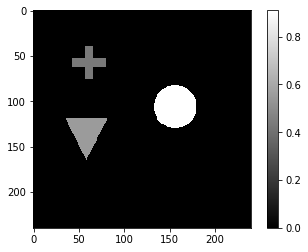
\includegraphics[width=\linewidth]{chapters/02_methods/images/rise/rise_original.png}
        \caption{Original image}
    \end{subfigure}\hfill%
    \begin{subfigure}[t]{.32\textwidth}
        \centering
        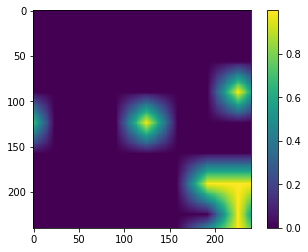
\includegraphics[width=\linewidth]{chapters/02_methods/images/rise/rise1_mask.png}
        \caption{RISE mask}
    \end{subfigure}\hfill%
    \begin{subfigure}[t]{.32\textwidth}
        \centering
        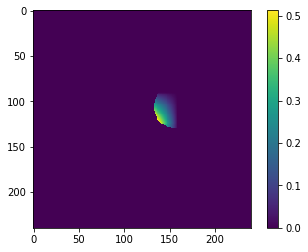
\includegraphics[width=\linewidth]{chapters/02_methods/images/rise/rise1_applied.png}
        \caption{RISE mask applied to original image by multiplication}
    \end{subfigure}
    \caption{By multiplication the input image (left) with a RISE mask (center), a modified input is generated (right). In comparison fo Figure \ref{rise_mask0}, this input image retains much less information.}
    \label{rise_mask1}
\end{figure}

The number of generated masks depend on the image resolution, e.g. for an image of size 240x240 pixels, 3000 masks generate good results. All masks are applied to the input image to generate new input images. The modified images are passed through the neural network and their classification scores for a specific class are recorded. A high classification score for a class on a modified input image means that the pixels preserved by the mask are important for the classification.

To visualize the results, the classification scores and masks are summed up and converted into a heat map. Figure \ref{rise_explanation} shows how the summing up works: The masks are multiplied with the classification score returned by running the masked image through the neural network. In Figure \ref{rise_explanation} for example, the leftmost mask was applied to an image, the image was run through the network and the network returned the value 0.7 for the first class. The next step is summing up all the values from the same cell into one matrix (image (c) in Figure \ref{rise_explanation}). In the actual implementation, the multiplication of the masks with the output values and summing up into one matrix is done with one matrix multiplication step.

\begin{figure}[H]
    \centering
    \begin{subfigure}[t]{\textwidth}
        \centering
        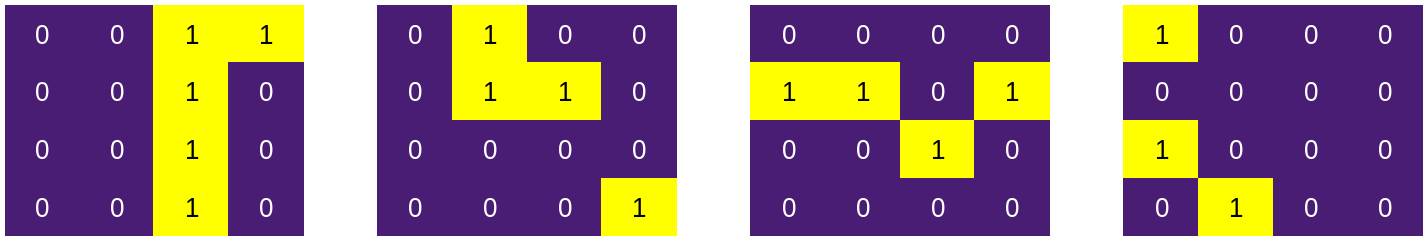
\includegraphics[width=\linewidth]{chapters/02_methods/images/rise/explain_rise_masks.png}
        \caption{Sample RISE masks}
    \end{subfigure}
    \begin{subfigure}[t]{\textwidth}
        \centering
        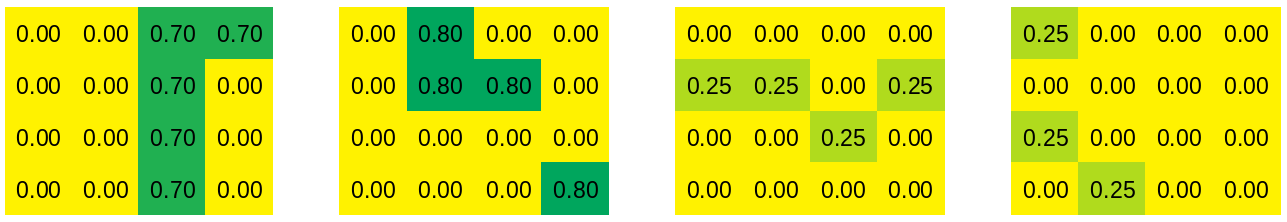
\includegraphics[width=\linewidth]{chapters/02_methods/images/rise/explain_rise_result.png}
        \caption{Masks multiplied by the classification value returned by the neural network after running the masked images through it}
    \end{subfigure}\hfill
    \begin{subfigure}[t]{.5\textwidth}
        \centering
        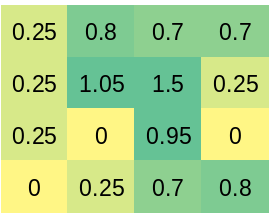
\includegraphics[width=\linewidth]{chapters/02_methods/images/rise/explain_rise_saliency.png}
        \caption{Saliency map generated by summing up all values for the same cell of the results in (b). E.g. second row second column is 0 + 0.8  + 0.25 + 0 = 1.05.}
    \end{subfigure}
    \caption{RISE masks (a) are multiplied by classification value returned by the network for the masked images (b). The same cell in theses matrices are summed up to generate a new matrix (c).}
    \label{rise_explanation}
\end{figure}

To visualize the generated matrix, the data is upscaled to the original image size and displayed as a heatmap by mapping the values to a color map. Figure \ref{rise_example} shows some examples for visualization of the RISE output for specific classes.

\begin{figure}[H]
\centering
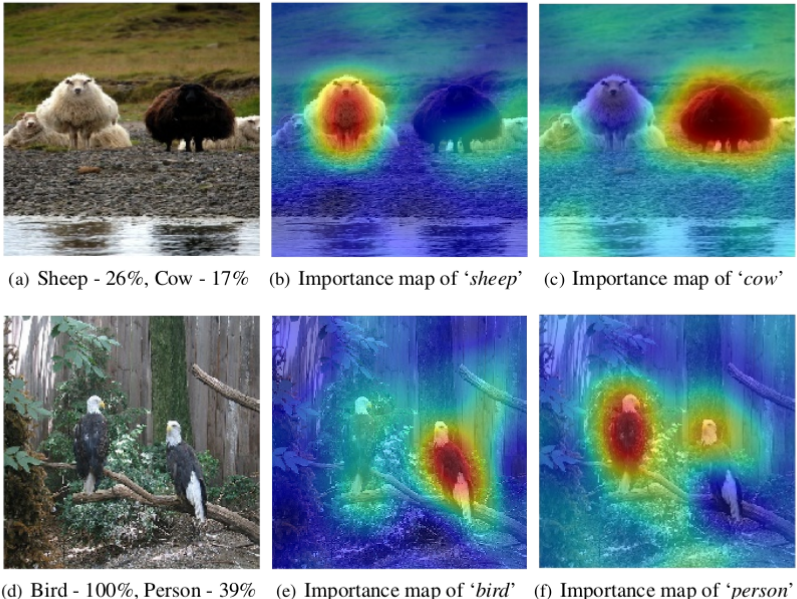
\includegraphics[width=12cm]{chapters/02_methods/images/rise/sheep.png}
\caption{Image from original paper explaining some classes}
\label{rise_example}
\end{figure}

\section{Grad-CAM}
Grad-CAM\cite{selvaraju2017grad} (Gradient-weighted Class Activation Mapping) is a white box method, it requires insight into the convolutional neural network architecture and is therefore only applicable on CNNs. The method generates a heat map similar to RISE. Figure \ref{grad_cam_cat} and Figure \ref{grad_cam_dog} are outputs of Grad-CAM on an example image.

\begin{figure}[H]
    \centering
    \begin{subfigure}{.5\textwidth}
        \centering
        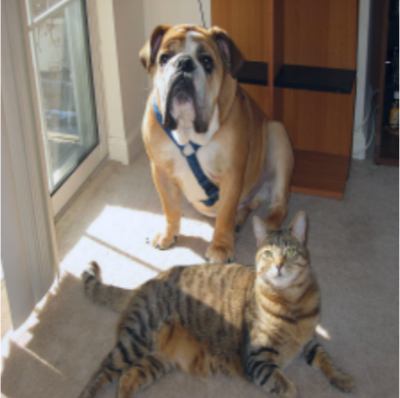
\includegraphics[width=0.7\linewidth]{chapters/02_methods/images/grad-cam-original.png}
        \caption{Original image}
    \end{subfigure}\hfill%
    \begin{subfigure}{.5\textwidth}
        \centering
        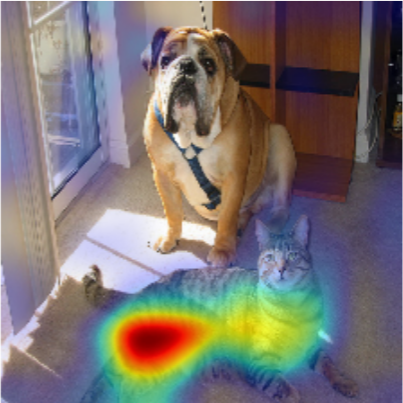
\includegraphics[width=0.7\linewidth]{chapters/02_methods/images/grad-cam-cat.png}
        \caption{Grad-CAM explanation for class cat}
    \end{subfigure}
    \caption{Grad-CAM applied on an image with multiple valid classes. Explanation for class cat.}
    \label{grad_cam_cat}
\end{figure}

\begin{figure}[H]
    \centering
    \begin{subfigure}{.5\textwidth}
        \centering
        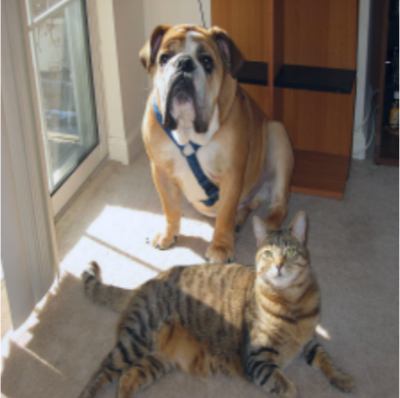
\includegraphics[width=0.7\linewidth]{chapters/02_methods/images/grad-cam-original.png}
        \caption{Original image}
    \end{subfigure}\hfill%
    \begin{subfigure}{.5\textwidth}
        \centering
        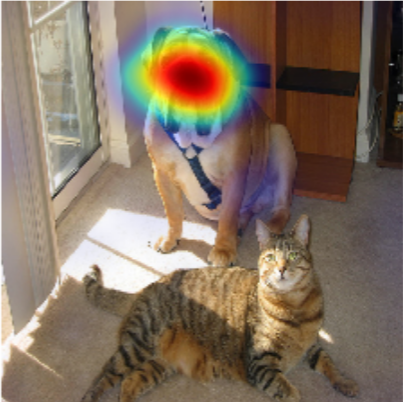
\includegraphics[width=0.7\linewidth]{chapters/02_methods/images/grad-cam-dog.png}
        \caption{Grad-CAM explanation for class dog}
    \end{subfigure}
    \caption{Grad-CAM applied on an image with multiple valid classes. Explanation for class dog.}
    \label{grad_cam_dog}
\end{figure}

The main parameter for this method is which convolutional layer of the neural network that should be analyzed. Figure \ref{grad_cam_explanation} shows a schematic of the inner working of Grad-CAM for a layer: The feature map (i.e. the result of applying the convolution kernels on the channel input) of the specified convolutional layer is extracted. Every channel of the feature map is weighted, based on how much it influences the final output value of the network for a specific class. Finally, the weighted channels are summed up, run trough ReLU and converted to a heat map by upsamling. The ReLU is applied to remove pixels which negativly impact the class output.

\begin{figure}[H]
\centering
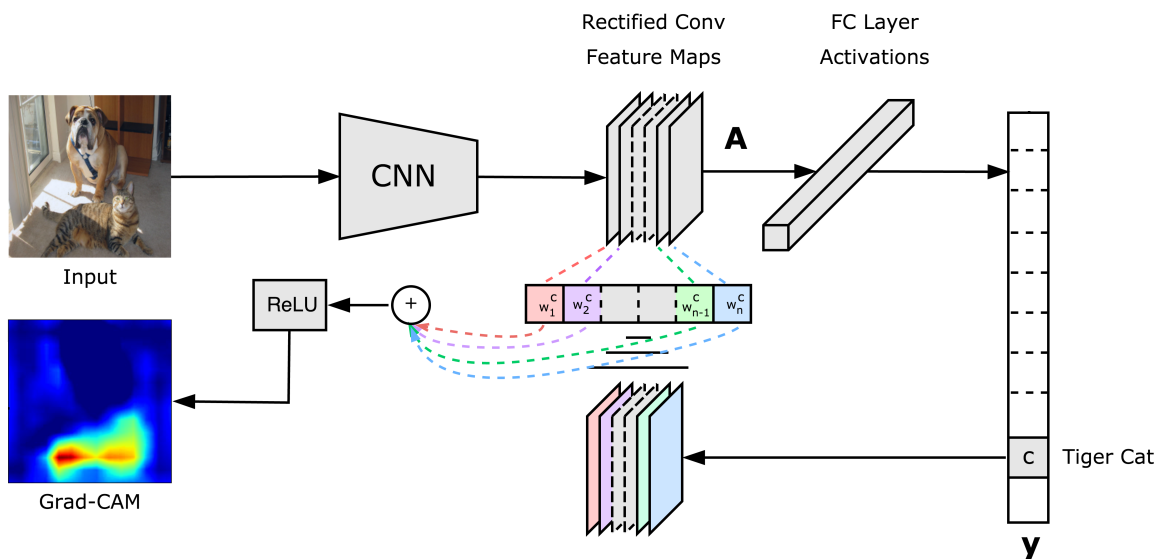
\includegraphics[width=12cm]{chapters/02_methods/images/grad-cam.png}
\caption{Grad-CAM in action: The feature map of a specific network layer is extracted, each channel weighted by the activation of the expected class, summed up and converted into a heat map}
\label{grad_cam_explanation}
\end{figure}



\chapter{Classification}
\section{NIH Chest X-ray dataset}
To find out what outputs the different methods generate, we started with a simple classification task in the medical image field:

\section{Model Training}






\subsection{Inception Resnet v2}
\begin{itemize}
    \item  chest x-ray, sample data set (small subset)
    \item  multi label classification
    \item  current state of the art networkj: inception  resetnet v2 (accurate + fast to train on single GPU) \cite{todo}
    \item  using learnings and code from project2
    \item  slightly modified inception resnet v2 implementation (grayscale instead of color)
    \item  did not work, convert to RGB and downscale images (offline, preprocess.ipynb)
    \item  results: 40\% validation accuracy => bad
    \item smaller batch size (citation needed) 5, => not better
    \item next: use full dataset
    \item download 42 gigs of data
    \item simple python multiprocessing for preprocessing
\end{itemize}

\subsection{ResNet}
Instead of waiting for the expected very long learning time for Inception-Resnet V2, we did a short test with Resnet50 with pretrained parameters (ImageNet) on the sample dataset. Only the last layer is unfreezed.

\begin{itemize}
    \item Epoch time of ~40 seconds instead of (TODO) 10 minutes/3 hours for full dataset
    \item resnet50 with pretrained
    \item resnet50 without pretrained
    \item resnet18 without pretrained
    \item resnet18 without pretrained full dataset
\end{itemize}

\subsection{Only images with actual diagnosis}
https://www.kaggle.com/kmader/train-simple-xray-cnn 
For testing out the methods, images with findings are much more helpful, so filter them out.

Better results:


\subsection{Single label only}
65\%

\subsection{Densenet}
% https://medium.com/@jrzech/reproducing-chexnet-with-pytorch-695ff9c3bf66

Loading the saved model did not work, because the used version of PyTorch was old and incompatible with ours.

=> Retraining

\subsubsection{Image resize problems}
In the Densenet code there was a reference that some images were not properly resized. We did a short check on our preprocessed data, but it revelead no such problems. Used bash command:

\begin{minted}{bash}
find . -name '*.png' -exec file {} \; | cut -c 37-45 | uniq
\end{minted}

\subsection{Densenet single}
\begin{itemize}
    \item Fail: Not correctly setting up classes (last layer has 1000 classes for imagenet, we have 14)
    \item Fail 2: Train and validation set do not have same classes because of ordering in dataset loading code
\end{itemize}

After training for a short time with the fixes, we get an acceptable accuracy rate of 55\%. We then started to calculate the accuracy per class, as has been done on the reproduce-chexnet discussed above. We quickly discovered that only the "No findings" class was accurate, an all other classes had zero correct classifications.

\begin{itemize}
    \item test with no findings removed => not that better, finds only 3 classes correctly
    \item try with weighted cross entropy loss
\end{itemize}



\section{Applying RISE}
Problem: returned classes from RISE do not match with precalculated classes
=> normalize was not applied on find\_best\_images.
=> use same function on all image loaders

\section{Applying LIME}
\section{Applying Grad-CAM}


\chapter{Segmentation}
\section{BraTS 2018 dataset}
\section{Medical background}
The scans in the BraTS 2018 datasets are created with four different settings of the MRI scanner:

GD-enhancing tumor (ET — label 4),
peritumoral edema (ED — label 2),
necrotic and non-enhancing tumor core (NCR/NET — label 1)

% https://www.researchgate.net/post/What_are_the_differences_between_enhancing_and_nonenhancing_lesions_in_MRI

The scanners detect three different types of kinds of tumor tissues. 
Gadolinium is a chemical compound given during MRI scans that highlights areas of inflammation (Active Lesions). A gadolinium-enhanced  MRI scan shows active lesions, meaning that there is a breakdown of the blood-brain barrier and inflammation is present.


\begin{itemize}
    \item Native (T1)
    \item Post-contrast T1-weighted (T1Gd)
    \item T2-weighted (T2)
    \item T2 Fluid Attenuated Inversion Recovery (FLAIR)
\end{itemize}

\section{Preprocessing \& Slice selection}
These are also saved as 2 byte integers with the values 0 (not tumor), 1 (todo), 2(todo) and 4(todo).

Every layer is saved as a 2 byte signed integer. We convert these to 1 byte unsigned integers and scale the range to 0-255, so the highest value in the 2 byte signed integer is 255 and the lowest is 0.
This way we generate a grayscale image that can be viewed with a normal image viewer and should be processable by a normal convolutional neural network

\section{Neural network architecture}
https://github.com/milesial/Pytorch-UNet
https://github.com/usuyama/pytorch-unet

modifications: do not use deprectated functions

\section{Training}

first try. baaad
second try with normalization: no change
build evaluation
third try with batch norm: much higher loss that slowy goes down, evaluate still shows random pixels
5. run it for some hours, it worked!

\section{Modifying and applying RISE (Single Pixel)}
\section{Modifying and applying RISE (Multi Pixel)}
\section{Modifying and applying Grad-CAM}


\chapter{Testnet}
\section{Motivation}



\section{Introduction}
\nblink{brats/08\_testnet\_generate.ipynb}
\nblink{brats/09\_testnet\_train.ipynb}

\section{Applying RISE}
\nblink{brats/brats/10\_testnet\_rise.ipynb}
\nblink{brats/brats/11\_testnet\_rise\_segment\_ignore.ipynb}


\subsection{Results}
TODO Multipixel RISE results

\subsection{Discussion}
TODO: something is visible, but not good enough


\chapter{Modified BraTS with tumor contours}
\section{Introduction \& Motivation}
\section{Applying RISE}

\chapter{Hausdorf Distance masks}
\section{Introduction}
\section{Hausdorff distance}
\section{Masking}
\section{Visualization}
\section{Applying HDM on Testnet}
\section{Applying HDM on BraTS}
\section{Applying HDM on modified BraTS}
\section{Applying HDM on BraTS 3D}

\chapter{Infrastructure \& tooling}
\section{Infrastructure setup}
Computer reachable from internet, running jupyter with password,
rtx 2080

\section{Scripts}

\section{Testing}


\chapter{Discussion}
compare with requirements document

\chapter{Conclusion}